% =========================================================================== %
% Introduction
% =========================================================================== %

\ifx\wholebook\relax\else
  \documentclass[a4paper,10pt,twoside]{book}
  %=============================================================================%
% Common things, settings, packages to include
%=============================================================================%

\usepackage{graphicx}
\usepackage{color}
\usepackage{makeidx}
\usepackage{ifpdf}
\usepackage{verbatim}

% --------------------------------------------------------------------------- %
% Setting up stuff depeding on output format
% --------------------------------------------------------------------------- %

\ifpdf
  % special settings for pdf mode
  \usepackage[colorlinks]{hyperref}
  \usepackage{courier}
  
  \hypersetup{
    colorlinks,
    linkcolor=darkblue,
    citecolor=darkblue,
    pdftitle={The Eclipse Scout Book},
    pdfauthor={The Scout Community},
    pdfkeywords={Enterprise Framework, Eclipse, Java, Client-Side, Rich Client, Web Client, Mobile},
    pdfsubject={Computer Science}
  }
  
  \usepackage{caption}
  \captionsetup{margin=10pt,font=small,labelfont=bf}
\else
  % special stuff for html mode
  \usepackage[tex4ht]{hyperref}
\fi

% --------------------------------------------------------------------------- %
% Setting up printing range
% --------------------------------------------------------------------------- %

\parindent 1cm
\parskip 0.2cm
\topmargin 0.2cm
\oddsidemargin 1cm
\evensidemargin 0.5cm
\textwidth 15cm
\textheight 21cm

% --------------------------------------------------------------------------- %
% Setting up listings
% --------------------------------------------------------------------------- %

\usepackage{listings}
 
\definecolor{darkviolet}{rgb}{0.5,0,0.4}
\definecolor{darkgreen}{rgb}{0,0.4,0.2} 
\definecolor{darkblue}{rgb}{0.1,0.1,0.9}
\definecolor{darkgrey}{rgb}{0.5,0.5,0.5}
\definecolor{lightblue}{rgb}{0.4,0.4,1}
\definecolor{lightgray}{rgb}{0.97,0.97,0.97}

\renewcommand{\lstlistlistingname}{List of Listings}

% general settings
\lstset{
  basicstyle=\small\ttfamily,
  columns=fullflexible,
  breaklines=true,
  breakindent=10pt,
  prebreak=\mbox{{\color{blue}\tiny$\searrow$}},
  postbreak=\mbox{{\color{blue}\tiny$\rightarrow$}},
  showstringspaces=false,
  backgroundcolor=\color{lightgray}
}

% settings for xml files
\lstdefinelanguage{xml}
{
  commentstyle=\color{darkgrey}\upshape,
  morestring=[b]",
  morestring=[s]{>}{<},
  morecomment=[s]{<?}{?>},
  stringstyle=\color{black},
  identifierstyle=\color{darkblue},
  keywordstyle=\color{cyan},
  morekeywords={xmlns,name,point,factory,class}% list your attributes here
}

% settings for ini files
\lstdefinelanguage{ini}
{
  morecomment=[f][\color{darkgrey}\upshape][0]\#, % # is comment iff it's the first char on the line
  stringstyle=\color{black}
}

% default settings (for java files)
\lstset{
  language=Java,
  emphstyle=\color{red}\bfseries,
  keywordstyle=\color{darkviolet}\bfseries,
  commentstyle=\color{darkgreen},
  morecomment=[s][\color{lightblue}]{/**}{*/},
  stringstyle=\color{darkblue},
}

% --------------------------------------------------------------------------- %
% cross reference macros
% --------------------------------------------------------------------------- %
\newcommand{\applabel}[1]{\label{apx:#1}}
\newcommand{\chalabel}[1]{\label{cha:#1}}
\newcommand{\seclabel}[1]{\label{sec:#1}}
\newcommand{\lstlabel}[1]{\label{lst:#1}}
\newcommand{\figlabel}[1]{\label{fig:#1}}
\newcommand{\tablabel}[1]{\label{tab:#1}}

\newcommand{\appref}[1]{Appendix~\ref{apx:#1}}
\newcommand{\charef}[1]{Chapter~\ref{cha:#1}\xspace}
\newcommand{\secref}[1]{Section~\ref{sec:#1}}
\newcommand{\lstref}[1]{Listing~\ref{lst:#1}\xspace}
\newcommand{\figref}[1]{Figure~\ref{fig:#1}\xspace}
\newcommand{\tabref}[1]{Table~\ref{tab:#1}\xspace}

% --------------------------------------------------------------------------- %
% graphics paths
% --------------------------------------------------------------------------- %
\graphicspath{
  {figures/}
  {Introduction/figures/}
}

%=============================================================================%

  \pagestyle{headings}
  \graphicspath{{figures/} {../figures/}}
  \begin{document}
  \sloppy
\fi


% =========================================================================== %
\chapter{Introduction}

% --------------------------------------------------------------------------- %
\section{What is Eclipse Scout?}

\fbox{
  \parbox{12cm}{
    Section waiting for contribution (max 2'000 words)
	
    The focus of the first section should be on benefits of Scout.
	History should point to the 10 years of existence of Scout and previous technology transitions.
	Outlook should focus on values such as stability, dedication to grow the community and moving with best available technolgies.
  }
}

\noindent Existing Documentation
\begin{itemize}
  \item concept wiki \url{http://wiki.eclipse.org/Scout/Overview}
\end{itemize}

\subsection{Benefits of Scout}

\noindent Existing Documentation
\begin{itemize}
  \item concept wiki \url{http://wiki.eclipse.org/Scout/Overview/Why_You_Should_Use_Scout}
\end{itemize}

Eclipse Scout is a mature and open framework for modern, 
service oriented business applications.

With its multi-frontend support, Scout applications may run as desktop 
applications, in the web or on a mobile using a single codebase.

Scout substantially boosts developer productivity and is simple to learn.

User friendly applications are straight forward to implement with Scout�s 
comprehensive set of user interface components.

Completely based on Java/Eclipse, Scout Applications are easy to integrate 
in most IT environments.

\subsection{A short History}
needs text

\subsection{Outlook}
needs text

\newpage

% --------------------------------------------------------------------------- %
\section{What should I read?} 
\seclabel{whatshouldiread}

The text below provides guidelines on what to read (or what to skip) depending on your existing background.

We first address the needs of junior Java developers that like to learn more about developing enterprise applications.
Then, we suggest a list of sections relevant for software wizards that already have a solid understanding of the Eclipse platform, Java enterprise technolgies, and real world applications.
Finally, the information needs of IT managers are considered.

% ........................................................................... %
\subsection{I know some Java}

The good news first.
This book is written for you! 
No prior knowledge of the Eclipse Platform\footnote{Eclipse Platform: \url{http://wiki.eclipse.org/Platform}} is needed. 
We do not even assume that you have a meaningful understanding of the Java Enterprise Edition 
(Java EE)\footnote{Java Enterprise Edition: \url{http://en.wikipedia.org/wiki/Java_Platform,_Enterprise_Edition}}.
Of course, having prior experience in client server programming with Java is helpful.
It also helps having used the Eclipse IDE for Java development before --- please do not mistake the IDE with the Eclipse 
platform\footnote{By reading through the book you will learn that there is much more to the Eclipse platform than just the IDE}.
However, prior knowledge of Java EE and the Eclipse platform is not required for this book.

The ``bad'' news is, that writing Scout applications requires a solid understanding of Java.
To properly benefit from this book, we assume that you have been developing software for a year or more.
And you should have masterd the Java Standard Edition 
(Java SE)\footnote{Java Standard Edition: \url{http://en.wikipedia.org/wiki/Java_SE}} to a significant extent. 
To be more explicit, you are expected to be comfortable with all material required for the Java Programmer Level I 
Exam\footnote{Level I Exam: \url{docs.oracle.com/javase/tutorial/extra/certification/javase-7-programmer1.html}}
and most of the material required for 
Level II\footnote{Level II Exam: \url{docs.oracle.com/javase/tutorial/extra/certification/javase-7-programmer2.html}}.

As the focus of this book is on writing Scout applications and not on learning Java, Java EE, or the Eclipse platform, the necessary background material has been moved into corresponding appendices.
To get a more precise picture which parts of Java and Eclipse are important to Scout applications, consult the appendices listed below.

\begin{itemize}
  \item \appref{java_basics} highlighs relevant advanced Java SE concepts and necessary Java EE topics. 
        In addition, the appendix contains recommendations for introductory material as well as pointers to further reading regarding Java EE technology.
  \item \appref{eclipse_basics} provides a brief introduction for Eclipse concepts used in Scout. 
        This includes the OSGi/Equinox foundation as well as additional elements such as Eclipse plugins, feature and product files.
\end{itemize}

We now propose to start downloading and installing Scout as described in \appref{install_scout} and do some actual coding.
To do so, please continue with the ``Hello World'' example provided in \charef{helloworld}.
You can expect to complete this example in less than two hours including the necessary download and installation steps.
Afterwards, you might want to continue with the remaining material in ``Getting Started''. 
Working through the complete ``Getting Started'' should take no more than two days. 
This exercise will provide you with a broad overview of Eclipse Scout and enough hands-on material to decide how much Scout will help you with your current and future projects.

How you continue after ``Getting Started'' will depend on your current interests or your specific project. 
``The Frontend'' and ``The Backend'' walk you through the Scout application model covering the client, the server, and the necessary communication in the context of a typical business application.
``Developing Applications'' contains additional Scout features, relevant aspects for integrating Scout applications in an enterprise envrionment, and typical topics important to professional software development.

Once you work with the Scout framework on a regular basis, you might want to ask questions in the Scout 
forum\footnote{Eclipse Scout forum: \url{http://www.eclipse.org/forums/eclipse.scout}}.
When your question gets answered, please ask yourself if your initial problem could have been solved by better documentation.
In that case, you might want to help the Scout community by fixing or amending the Scout wiki pages\footnote{Eclipse Scout wiki: \url{http://wiki.eclipse.org/Scout}}.
Or this book. 
If you find a bug in Eclipse Scout that makes your life miserable you can report it. 
When your bug is fixed, you can test the fix.
To help speed up the bugfixing process you can contribute patches.
All of these actions will add to the healthy grow of the Scout community.
And this is exactly the topic of ``Contributing'', the last part of this book.

% ........................................................................... %
\subsection{I know tons of both Java and Eclipse}

This means that you are one of these software wizards that get easily bored.
You probably hate going through lengthy descriptions of widely known concepts.
In that case let us assume that you are prepared to spend two hours to grasp the scope of Eclipse Scout and get an impression of its strengths and limitations.

In that case you will not need to actually download, install, and code. 
Rather, it will suffice to flip through a couple of diagrams and screenshots, read about some central Scout concepts, and look at some code snippets provided in this book.
The list below suggests a sequence of sections to digest including a brief motivation for each one.

\begin{itemize}
  \item \prtref{getting_started} ``Getting Started'' 
      Provides you with the big picture. Skip the larger example in \charef{large_example}
  \item \charef{client_overview} ``Overview'' and \charef{client_modeling} ``Client Modeling''
      Get familiar with the Scout frontend architecture and client modeling makes Scout applications independent of any particular user interface technology
  \item \charef{fields} ``Form Fields'' and \charef{custom_fields} ``Custom Fields''
      Browse through the screensthos in \charef{fields} to get an impression over the form fields that are available out of the box. 
	  Look at the diagrams in \charef{custom_fields} to get an idea of how to extend the Scout framework with missing field types.
  \charef{server_overview} ``Overview'', \charef{services} Scout server
  % \item read overview and transaction management in backend
  % \item read application extensions to learn how scout applications can be properly modularized 
  % \item maybe check how to use your favorite logging framework with scout
  % \item glance at web and mobile application to learn how scout can use a single codebase to run an application on the desktop in the web, and on mobile devices
  % \item glance over the shocase sections in "integrating 3rd party" to see how scout applications integrate with other frameworks
  % \item flip though testing/profiling to convince yourself that developing scout applications is not different from developing other java/eclise applications	
\end{itemize}

% \begin{itemize}
  % \item read ''getting started'' but skip the larger example
  % \item read overview and client modeling in frontend 
  % \item flip though the form fields provided out of the box
  % \item maybe check custom fields to see how to add missing form fields
  % \item read overview and transaction management in backend
  % \item read application extensions to learn how scout applications can be properly modularized 
  % \item maybe check how to use your favorite logging framework with scout
  % \item glance at web and mobile application to learn how scout can use a single codebase to run an application on the desktop in the web, and on mobile devices
  % \item glance over the shocase sections in "integrating 3rd party" to see how scout applications integrate with other frameworks
  % \item flip though testing/profiling to convince yourself that developing scout applications is not different from developing other java/eclise applications	
% \end{itemize}

% ........................................................................... %
\subsection{I am a manager}

Beeing a manager and actually reading this book may indicate one of the following situations:

\begin{itemize}
  \item Your developer tried to convince you that Eclipse Scout can help you with implementing business applications in a shorter time and for less money.
        And you did not understand why (again) a new technology should work better than the ones you already use. 
	
\end{itemize}

% =========================================================================== %
\chapter{''Hello World''}
\chalabel{helloworld}

The ''Hello World'' chapter walks you through the creation of an Eclipse Scout client server application.

This ''Hello World'' application will work the following way.
When the user starts the client part of this Scout application, the client connects to the server\footnote{
For the intended scenario, the Scout server part of the ''Hello World'' application will be running on a webserver.
} 
and asks for some text content that is to be displayed to the user.
Next, the server retrives the desired information and sends it back to the client.
The client then copies the content obtained from the server into a text field widget.
Finally, the client displays the message obtained from the server in a text field widget.

The goal of this chapter is to provide a first impression of working with the Scout framework using the Scout SDK.
We will start by building the application from scratch and then we'll deploy the complete application to a Tomcat webserver.
Except for a single line of code in the server part of the ''Hello World'' application, we will only be using the tooling provided by the Scout SDK.

\fbox{
  \parbox{12cm}{
\noindent Existing Documentation
\begin{itemize}
  \item wiki tutorial \url{http://wiki.eclipse.org/Scout/Tutorial/3.8/HelloWorld}
\end{itemize}
  }
}
% --------------------------------------------------------------------------- %
\section{Installation and Setup}

Before you can start with the Scout ''Hello World'' example you need to have a complete and working installation.
See the step-by-step installation guide provided in \appref{install_scout}.
Once you have everything installed, you are ready to create your first Scout project.

% --------------------------------------------------------------------------- %
\section{Create a new Project}
\seclabel{create_project_simple}

Start your Eclipse IDE and select an empty directory for your 
workspace\footnote{The term \textit{workspace} is used for a directory containing the relevant project artefacts such as the Java souce files or configuration files.} 
as described in \secref{download_install}.
To create a new Scout project, either select the \contextmenu{New Scout Project...} as shown in \figref{sdk_create_new_scout_project} or use the Eclipse \menu{File|New|Project...}.
In the latter case you are shown the generic \wizard{New Project} of Eclipse.
On the first dialog step, select the \wizard{Scout Project} below the Scout folder as seen in \figref{sdk_new_project_wizard}.
With the \button{Next} you will be directed to the next dialog step, the \wizard{New Scout Project}.

\begin{figure}
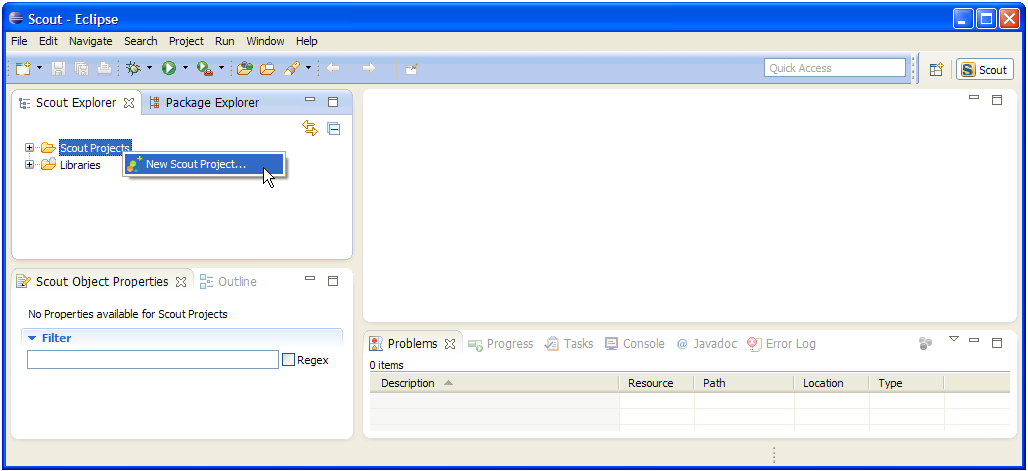
\includegraphics[width=13cm]{sdk_create_new_scout_project.png}
\caption{Create a new Scout project}
\figlabel{sdk_create_new_scout_project}
\end{figure}

In the \wizard{New Scout Project} you first enter a name for you Scout project. 
As we are creating a ''Hello World'' application, use \texttt{org.eclipse.scout.helloworld} for the \field{Project Name}.
As shown on the right hand side of \figref{sdk_new_project_wizard}, the wizard will automatically use the part after the last period of the project name as the application alias. 
(TODO: explain what the project alias is used for. E.g. in development server servlet is usually mapped to http://localhost:8080/''alias''/). 
Now, click the \button{Finish} to let the Scout SDK create the initial project code for you.

\begin{figure}
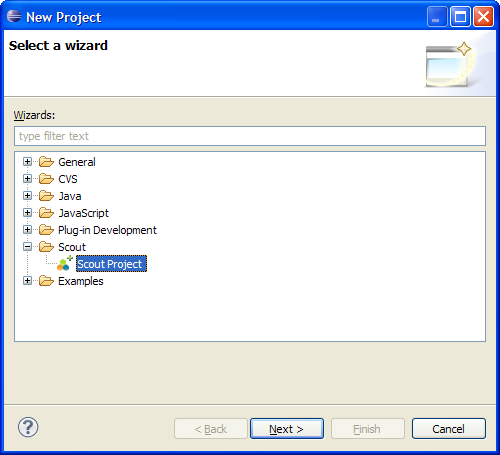
\includegraphics[width=7cm]{sdk_new_project_1.png} \hspace{5mm}
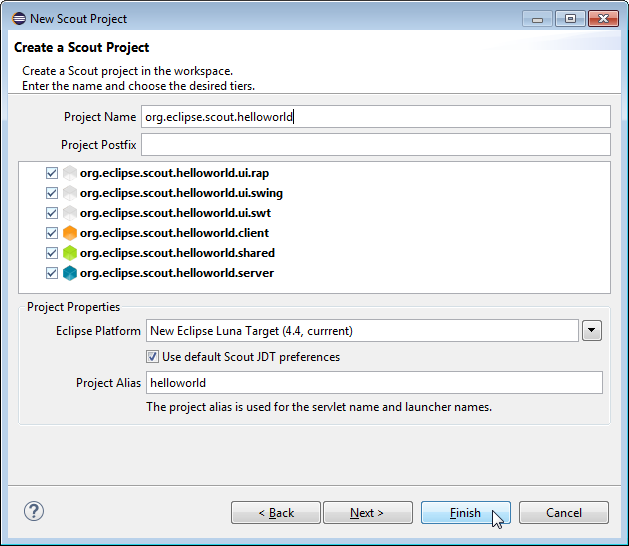
\includegraphics[width=7cm]{sdk_new_project_2.png}
\caption{The new project wizard. The dialog on the left side is only shown when using the generic \wizard{New Project} of Eclipse}
\figlabel{sdk_new_project_wizard}
\end{figure}

\begin{figure}
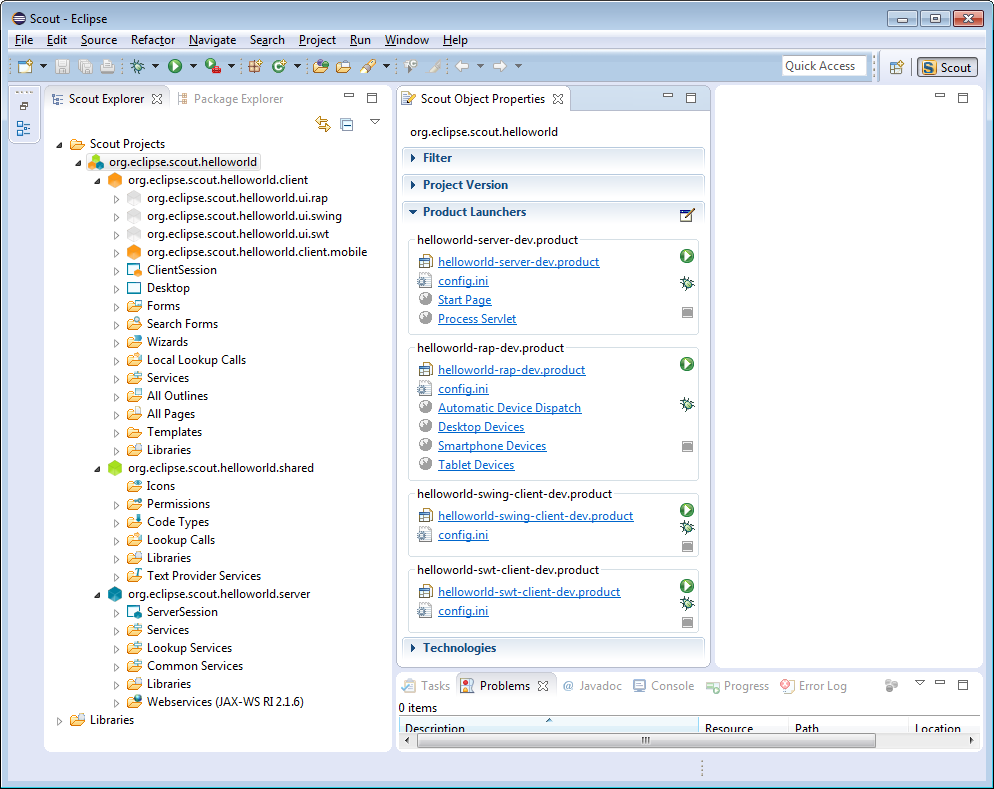
\includegraphics[width=13cm]{sdk_initial_helloworld_project.png}
\caption{The Scout SDK showing the tree representation of our ''hello world'' application in the Scout Explorer.
Scout Object Properties displays the product launchers for the server and the available clients.}
\figlabel{sdk_initial_helloworld_project}
\end{figure}

Once the initial project code is built, the Scout SDK displays the application model in the \textit{Scout Explorer}.
This model is visually presented as a tree structure covering both the client and the server part of the application.
In \figref{sdk_initial_helloworld_project} the Scout Explorer displays the top level elements of the complete Scout application.
Selecting the application's root node \texttt{org.eclipse.scout.helloworld} in the Scout Explorer displays the product launchers in the \textit{Scout Object Properties}.
As we can see in \figref{sdk_initial_helloworld_project}, we have shortcut icons to launch and stop four different development 
products\footnote{Product files define all the necessary elements of an application.}.

\begin{itemize}
  \item \textbf{Server}: the server application
  \item \textbf{Swing}: the Swing client application
  \item \textbf{SWT}: the SWT client application
  \item \textbf{RAP}: the RAP server application
\end{itemize}

The server box provides links to the Eclipse product file \texttt{helloworld-server-dev.product}, the server configuration file \texttt{config.ini} as well as three icons to launch and stop the Scout server in the Scout SDK.
The same layout is used for controlling the other three products.
Both the Swing and the
SWT\footnote{Standard Widget Toolkit (SWT): \url{http://en.wikipedia.org/wiki/Standard_Widget_Toolkit}.} 
boxes represent rich clients\footnote{Rich client: \url{http://en.wikipedia.org/wiki/Fat_client}} 
that run on the desktop.
The RAP server application is used to enable Scout application to run in a browser, a tablet, or a mobile device.
RAP\footnote{Remote Application Platform (RAP): \url{http://www.eclipse.org/rap/}} is a framework that allows to use Java for server-side 
Ajax\footnote{Asynchronous JavaScript and XML (AJAX): \url{http://en.wikipedia.org/wiki/Ajax_\%28programming\%29}}.

\fbox{
  \parbox{12cm}{
\noindent Existing Documentation
\begin{itemize}
  \item how-to wiki \url{http://wiki.eclipse.org/Scout/HowTo/3.8/Create_a_new_project}
\end{itemize}
  }
}

% --------------------------------------------------------------------------- %
\section{Run the Initial Application}
\seclabel{run_initial}

After the initial project creation we are ready to start the empty Scout application.
For this, we switch to the Scout Explorer and select the root node \element{org.eclipse.scout.helloworld}.
This loads the applications properties into the Scout Object Properties inlcuding the product launcher section.
There, we start the Scout server using the green launcher icons highlighted in \figref{start_server}.

\begin{figure}
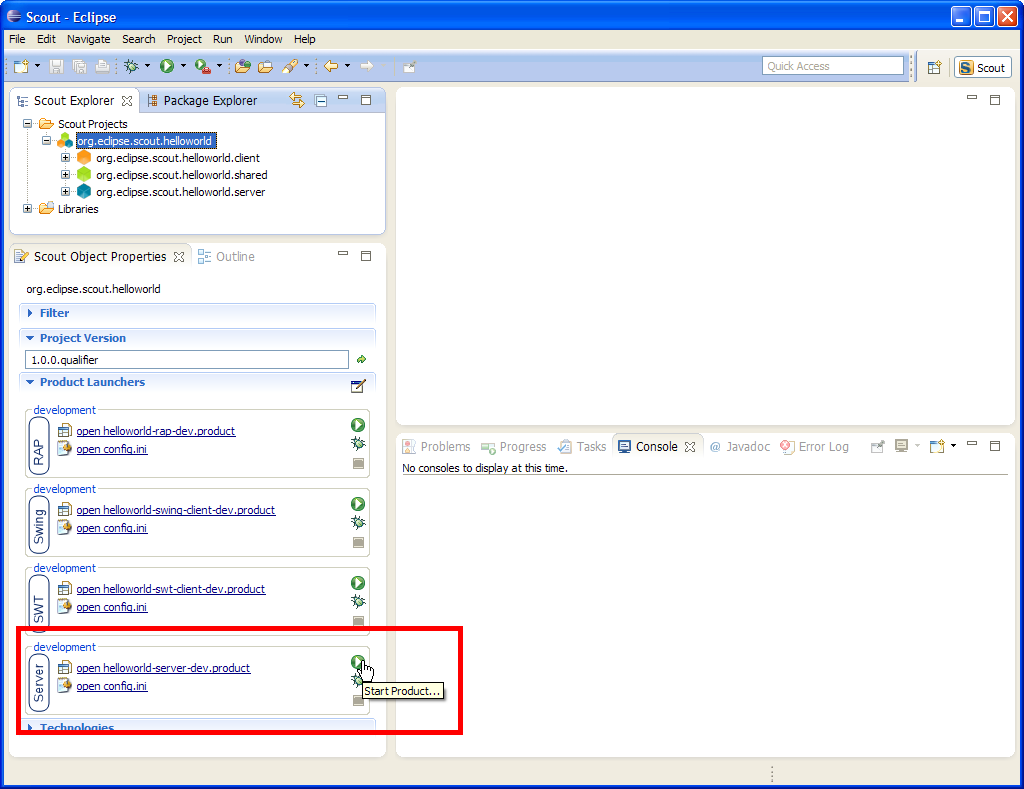
\includegraphics[width=13cm]{sdk_start_server_product.png} 
\caption{Starting the server application in the Scout SDK.}
\figlabel{start_server}
\end{figure}

Once the server is running, you may start the Swing client, the SWT client, and the RAP server in the same way.
To dispay the Scout client in a web browser, type the address \texttt{http://localhost:8082/web} into the browser's navigation bar.
You should then see the three different clients with an empty desktop on each as shown in \figref{helloworld_empty}.

\begin{figure}
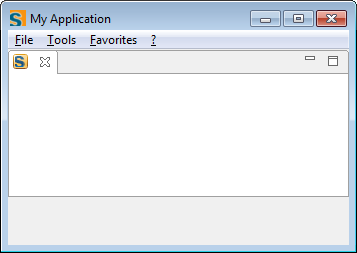
\includegraphics[width=4.5cm]{hellworld_empty_swing.png} \hspace{3mm}
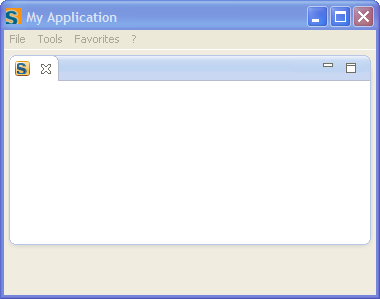
\includegraphics[width=4.5cm]{hellworld_empty_swt.png} \hspace{3mm}
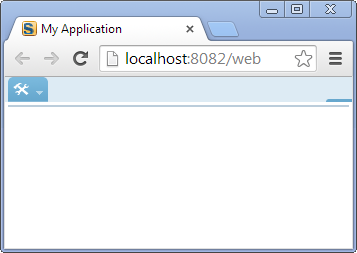
\includegraphics[width=4.5cm]{hellworld_empty_rap.png}
\caption{Running the three empty client applications from the Scout SDK. From left to right: The Swing client, the SWT client, and the webclient}
\figlabel{helloworld_empty}
\end{figure}

% --------------------------------------------------------------------------- %
\section{Walking through the Initial Application}

In this section, we walk you through the central pieces of the generated initial application. 
This exercise will introduce you to important elements of the Scout application model.
A basic understanding of these model elements will help you understand the structure and working of the ''Hello World'' application.

\begin{itemize}
  \item Desktop
  \item Form
  \item Form handler
  \item Process service
  \item Form data
  \item Form field
\end{itemize}

Each of the above elements is represented by a Java class in Scout.
This allows us to explain the basic concept using our ''Hello World'' source code.
Please note, that all this Java code has been added in the project creation step by the Scout SDK described in \secref{create_project_simple}.
This implies that you are free to adapt/change this code according to your needs.

\subsection{Desktop}

The desktop is the central container of all visible elements of the Scout client application.
It inherits from Scout class \java{AbstractDesktop} and represents the empty application frame with attached elements, such as the applications menu tree.
In the ''Hello World'' application, it is the Desktop that is first opened when the user starts the client application.

To find the desktop class in the Scout Explorer, we first navigate to the orange \node{client} and double click the \node{Desktop} just below.
This will open the associated Java file \texttt{Desktop.java} in the editor view of the Scout SDK.
Of interest is the overwritten callback method \java{execOpend} shown in \lstref{helloworld.execopend}.

\lstinputlisting[
  label=\lstlabel{helloworld.execopend},
  caption=Creating and starting a form in the client's Desktop callback method \java{execOpened}.,
  index={DesktopForm},
  linerange={42-47},
  float
]
{../code/helloworld/org.eclipse.scout.helloworld.client/src/org/eclipse/scout/helloworld/client/ui/desktop/Desktop.java}

Method \java{execOpend} is called by the Scout framework after the desktop frame becomes visible.
The only thing that happens here is the creation of a \java{desktopForm} object, that gets assigned an icon before it is started via method \java{startView}.
This desktop form object is will later hold the text widget that is to be displayed to the user\footnote{
In the Scout application model we can only add UI fields to Scout form elements, not directly to the desktop.
}.
More information regarding form elements are provided in the next section.

\subsection{Form}
\seclabel{helloworld.form}

Scout forms are UI containers that hold form field widgets.
A Scout form always inherits from Scout class \java{AbstractForm} and can either be displayed as a dialog in its own window or shown as a view inside of another UI container.
In the ''Hello World'' application a \java{DesktopForm} object is created and displayed as a view inside of the desktop element.

To find the desktop form class in the Scout Explorer, expand the orange \node{client}\footnote{
To expand elements (nodes, folders, etc.) in the Scout Explorer, use a double click on the element or a single click on the plus icon in front of the element.}.
Below this node, you will find the \folder{Forms}. 
Expand this folder to show the \element{DesktopForm} as shown in \figref{helloworld_viewhandler}.
In the Scout Object Property window in the screenshot, we can also see the \property{Display Hint}.
Its value is set to 'View' to display the desktop form as a view and not as a dialog in its own frame.

\begin{figure}
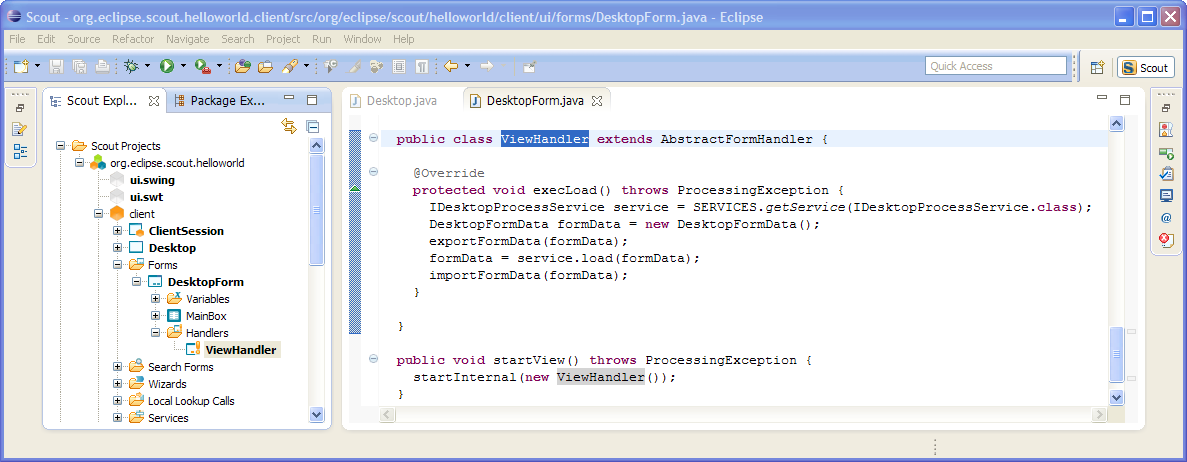
\includegraphics[width=15cm]{sdk_helloworld_viewhandler.png}
\caption{Scout SDK showing the DesktopForm's \textit{ViewHandler} in the Scout Explorer and the form properties in the Scout Object Properties.}
\figlabel{helloworld_viewhandler}
\end{figure}

Expand the \element{DesktopForm} to show its children: \element{Variables}, \element{MainBox} and \element{Handlers}.
The \element{Variables} subfolder contains variables. They are invisible to the application user.
The ''Hello World'' application is so simple, it does not need variables.
The subfolder \element{MainBox} contains form fields. These are the visible user interface elements.
Currently, the main box of our \java{DesktopForm} is empty. We will change this later.
Finally, the \element{Handlers} subfolder contains all available form handlers.
As shown in \figref{helloworld_viewhandler}, we already have a view handler available for our desktop form.

\subsection{Form Handler}
\seclabel{helloworld.formhandler}

Form handlers are used to manage the form's life cycle.
Scout form handlers inherit from \java{AbstractFormHandler} and allow the implementation of desired behaviour before a form is opend, or after it is closed.
This is achieved by overwriting callback methods defined in \java{AbstractFormHandler}.
The necessary wiring is provided by the Scout framework, either by the initial project creation step or when using one of the provided Scout SDK wizards.

\lstinputlisting[
  label=\lstlabel{helloworld.viewhandler},
  caption=Class \java{DesktopForm} with its view handler and \java{startView} method.,
  index={ViewHandler},
  emph={load},
  linerange={20-21,74-91},
  float
]
{../code/helloworld/org.eclipse.scout.helloworld.client/src/org/eclipse/scout/helloworld/client/ui/forms/DesktopForm.java}

In the ''Hello World'' application, it is the overwritten \java{execLoad} method in the \java{ViewHandler} (see \lstref{helloworld.viewhandler}) that defines what will happen before the desktop form is shown to the user.
This is the place where most of the behaviour relevant to the ''Hello World'' application is implemented.
Roughly, this implementation is performing the following steps.

\begin{enumerate}
  \item Get a reference to the process service running on the server.
  \item Create a data transfer object (DTO)\footnote{
Data Transfer Object (DTO): \url{http://en.wikipedia.org/wiki/Data_transfer_object}.}
  \item Pass the empty DTO to the load service method (ask the server for some data).
  \item Update the DTO with the content provided by the service method (use the answer provided by the server).
  \item Copy the updated information from the DTO into the desired form field.
\end{enumerate}

To open the \java{ViewHandler} class in the Java editor of the Scout SDK, double click on the \element{ViewHandler} in the Scout Explorer.
Your Scout SDK should then be in a state similar to \figref{helloworld_viewhandler}.
In the lower part of \lstref{helloworld.viewhandler} we can see the wiring between the desktop form and the view handler in method \java{startView}.
Further up, we find method \java{execLoad} of the view handler class.

Before we discuss this method's implementation, let us examine when and how \java{execLoad} is actually called.
As we have seen in the \java{Desktop} class (see \lstref{helloworld.execopend}), the form's method \java{startView} is executed after the desktop form is created.
Inside method \java{startView} (see \lstref{helloworld.viewhandler}), the desktop form is started/opened using \java{startInternal}.
In method \java{startInternal} a view handler is then created and passed as a parameter.
This eventually leads to the call of our \java{execLoad} custom implementation.

We are now ready to dive into the implementation of method \java{execLoad} of the desktop form's view handler.
First, a reference to a process service identified by \java{IDesktopProcessService} is obtained using \java{SERVICES.getService}.
Then, a form data object (the DTO) is created and all current form field values are exported into the form data via method \java{exportFormData}.
Strictly speaking, the \java{exportFormData} is not necessary for the use case of the ''Hello World'' application.
But, as this is generated code, there is no benefit when we manually delete the \java{exportFormData} command.
Next, using the \java{load} service method highlighted in \lstref{helloworld.viewhandler}, new form field values are obtained from the server and assigned to the form data object.
Finally, these new values are imported from the form data into the form via the \java{importFormData} method.
Once the desktop form is ready, showing it to the user is handled by the framework.

To add clarity and background to the implementation of the \java{execLoad} above, the next section introduces services and form data objects. 

\subsection{Process Services and Form Data Objects}

Process services and form data objects are used in the Scout framework to exchange information between client and server of a Scout application.
When needed, a service implemented on the server side can register a corresponding proxy service on the client.
This proxy service is invoked by the client as if it were implemented locally.
In fact, when we get a service reference using \java{SERVICES.getService}, we do not need to know if this service runs locally on the client or remotely on the server.

In the ''Hello World'' example application, the client's desktop form has an associated desktop process service running on the server.
This correspondence between forms and process services is also reflected in the \element{Links} section of the Scout Object Properties of the desktop form.
As shown in \figref{helloworld_viewhandler}, links are provided not only for the desktop form, but for its desktop form data, the corresponding desktop process service as well as for the process service interface \java{IDesktopProcessService}. 
On the client, this interface is used to identify and register the proxy service for the desktop process service.

To transfer data between the client and the server, the ''Hello World'' application uses a \java{DesktopFormData} object as a DTO.
This form data object holds all form variables and values for all the form fields contained in the form.
Taking advantage of this correspondence, the Scout framework provides the convenience methods \java{exportFormData} and \java{importFormData}.
As a result, the developer does not need to deal with any mapping code between the form data object and the form fields.

The actual implementation of the desktop process service in class \java{DesktopProcessService} is implemented on the server side.
As the class \java{DesktopProcessService} represents an ordinary Scout service it inherits from \java{AbstractService}.
It also implements its corresponding \java{IDesktopProcessService} interface used for registering both the actual service as well as the proxy service.

In \secref{helloworld.server} we will learn more about the desktop process service.

% --------------------------------------------------------------------------- %
\section{The User Interface Part}

In this section we will add the text field widget to the client's desktop form of the ''Hello World'' application.
In the steps described below, we use the \wizard{New Form Field} provided by the Scout SDK to add a group box field to the main box.
Then, we apply this wizard a second time on the group box to add the actual text widget\footnote{
Adding top level group boxes to a form helps in structuring the form layout, especially when a form contains a large number of form fields.
}.

To add the top level goup box to the main box, we first need to navigate to the \element{DesktopForm} in the Scout Explorer.
As explained in \secref{helloworld.form} every Scout form has a main box element that holds all form fields.
That is why we drill down to the \element{MainBox} element under the desktop form.
With a click of the right mouse button over the \element{MainBox} element in the Scout Explorer, the available context menues are displayed.
To start the new form field Scout wizard we select the \menu{New Form Field ...}.

\begin{figure}
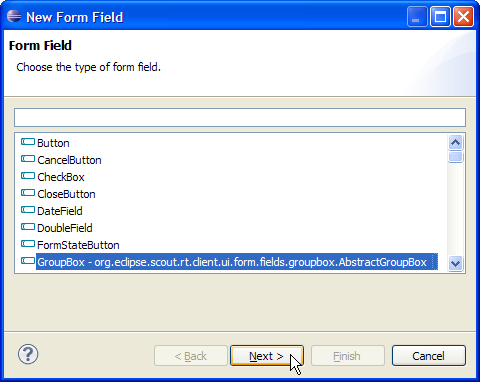
\includegraphics[width=7cm]{sdk_new_field_groupbox_1.png} \hspace{8mm}
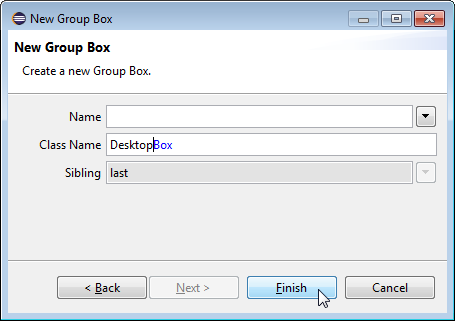
\includegraphics[width=7cm]{sdk_new_field_groupbox_2.png}
\caption{Adding the \textit{DesktopBox} field with the Scout SDK form field wizard.}
\figlabel{helloworld_groupboxfield}
\end{figure}

In the first dialog of the form field wizard shown in \figref{helloworld_groupboxfield}, we choose the form field type.
To select the desired field type, we either select the desired type with the mouse or use the serach field to filter the list of available field types.
In the second wizard dialog, we do not provide a label for the group box in the \field{Name}.
As we have only a single group box in the ''Hello World'' desktop form we omit the name and enter 'Desktop' into the \field{Class Name} before we close the wizard with the \button{Finish}.
The Scout SDK will add the necessary Java code for the \java{DesktopBox} in the background.

\begin{figure}
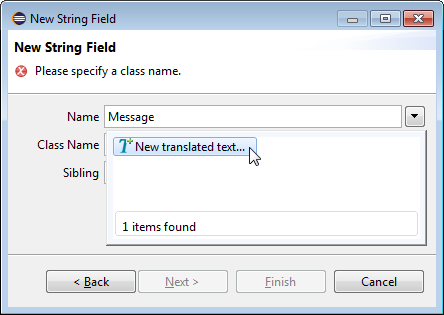
\includegraphics[width=6cm]{sdk_new_field_stringfield_1.png} \hspace{8mm}
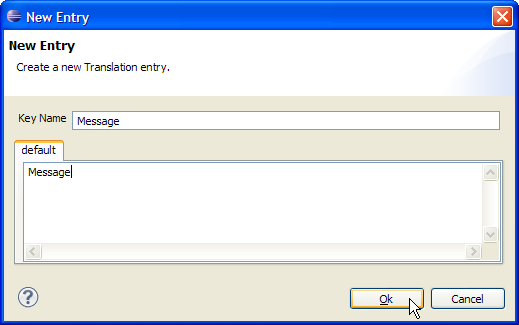
\includegraphics[width=7cm]{sdk_new_field_stringfield_2.png}
\caption{Adding a \textit{StringField} and providing a new translation entry.}
\figlabel{helloworld_stringfield}
\end{figure}

To add the text field widget to the group box, we first have to navigate to the newly created \element{DesktopBox} in the Scout Explorer.
On the desktop box (right below the main box element) we again use the \menu{New Form Field ...}.
In the first wizard dialog, we select \element{StringField} using 'st' as a search criteria and click the \button{Next} to open the second wizard dialog.
In the second wizard dialog, we enter 'Message' into the \field{Name}.
As we do not yet have the text 'Message' available in our ''Hello World'' application the wizard prompts the user with the proposal \textsc{New Translated Text ...} to add a new text entry as shown in \figref{helloworld_stringfield}.
This Scout SDK mechanism helps the developer to maintain the text keys separately from the actual text entries shown to the user that should never go directly into the applications source code and might get translated into different languages.
Once we have provided some initial translation for our message label, we can close the translation dialog with the \button{Ok}.
Finally, we close the form field wizard using the \button{Finish}.

\begin{figure}
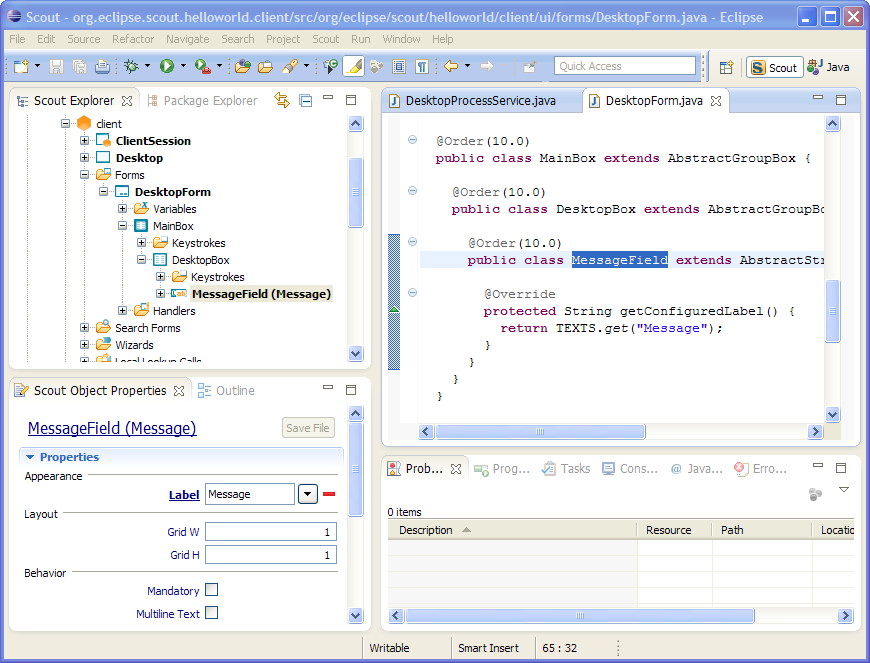
\includegraphics[width=12cm]{sdk_helloworld_messagefield.png}
\caption{Scout SDK showing the \it{MessageField}}
\figlabel{helloworld_messagefield}
\end{figure}

\lstinputlisting[
  label=\lstlabel{helloworld.mainbox},
  caption=The \java{MainBox} class with its desktop box and message field,
  index={MainBox},
  linerange={58-74},
  float
]
{../code/helloworld/org.eclipse.scout.helloworld.client/src/org/eclipse/scout/helloworld/client/ui/forms/DesktopForm.java}

When we drill down to the newly created message field in the Scout Explorer the Scout SDK should look similar to \figref{helloworld_messagefield}.
As shown in \lstref{helloworld.mainbox}, the message field and the desktop box field added with the \wizard{New Form Field} have been implemented as a structure of inner classes by the Scout SDK.
Using nested Java classes to model the form's content is a central aspect of the UI part of the Scout application model.
Among other benefits, it allows the Scout SDK to easily parse the form's Java code on the fly and directly reflect changes in the Scout Explorer and the Scout Property View.

Deriving the form model directly from the nested structure of inner classes also supports another important feature of the Scout SDK:
it keeps the form data classes in sync with the forms of the application.
This includes adding all the necessary getter and setter methods to access the values of all the fields defined on a form.
As a result, Scout developers don't need to update the form data objects after a form is changed.
The SDK takes care of this time consuming and error prone task.

% --------------------------------------------------------------------------- %
\section{The Server Part}
\seclabel{helloworld.server}

In this section we add the implementation of the \java{load} method of the \java{DesktopProcessService} defined on the server.
This is the last missing piece to complete the ''Hello World'' application.

As we have seen in \lstref{helloworld.viewhandler}, the \java{load} method of the desktop process service is called remotely from the client in the desktop form's view handler.
It is used by the client application to obtain some text content from the server that can then be shown to the user in the message widget\footnote{ 
The message widget is the field that we have added to the desktop form in the previous section.
}.

To navigate to the implementation of the desktop process service in the Scout SDK we first expand the blue top-level \node{server} in the Scout Explorer.
Below the server node, we further expand the \folder{Process Services} which shows the \element{DesktopProcessService} element.
Expand the \element{DesktopProcessService} node to show its \java{load} method.
This status of the Scout Explorer is also shown in \figref{helloworld_viewhandler}.

According to the signature of the \java{load} method, a desktop \java{formData} object is passed into this method that is then handed back to the caller in the return statement.
To complete the implementation of the \java{load} method it is sufficient to assign the text 'hello world' to the part of the form data that corresponds to the message field in the desktop form.
As we have learned in the previous section, the Scout SDK takes care of updating the form data when a form is changed.
This reduces the coding part of the ''Hello World'' application to the addition of the following statement:

\begin{lstlisting}[backgroundcolor=\color{white}]
  formData.getMessage().setValue("hello world!");
\end{lstlisting}

The complete implementation of the load method is provided in \lstref{helloworld.load}.
Even though this particular method looks simple and innocent, these process service methods are where the bulk of your server side code will end up.
This is the place where information obtained from databases, webservices (or completely different sources) is mapped to the UI elements presented to the user.
This is the place where information provided by the user is sent to webservices, saved in a database or processed in some way.

\lstinputlisting[
  label=\lstlabel{helloworld.load},
  caption=Assigning "hello world" to the form data's message field.,
  index={DesktopFormData,DesktopProcessService},
  linerange={10-14},
  float
]
{../code/helloworld/org.eclipse.scout.helloworld.server/src/org/eclipse/scout/helloworld/server/services/process/DesktopProcessService.java}

% --------------------------------------------------------------------------- %
\section{Add the Rayo Look and Feel}

In this section we will add Rayo to our ''Hello World'' Swing client application.
Rayo is slick look and feel for Scout desktop applications that is based on Swing.
As shown in \figref{helloworld_clientapp}, we get a Scout desktop application that looks the same as the corresponding Scout web client.

\begin{figure}
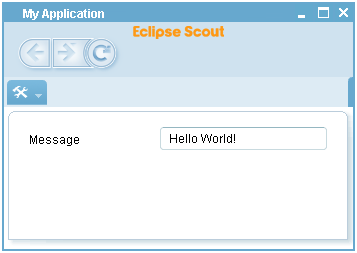
\includegraphics[width=7cm]{helloworld_message_swing_rayo.png} \hspace{5mm}
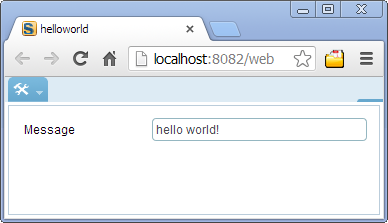
\includegraphics[width=7cm]{helloworld_message_rap_rayo.png}
\caption{The ''Hello World'' client application with the Rayo look and feel. The desktop client is shown on the left and the web client on the right hand side.}
\figlabel{helloworld_clientapp}
\end{figure}

\begin{figure}
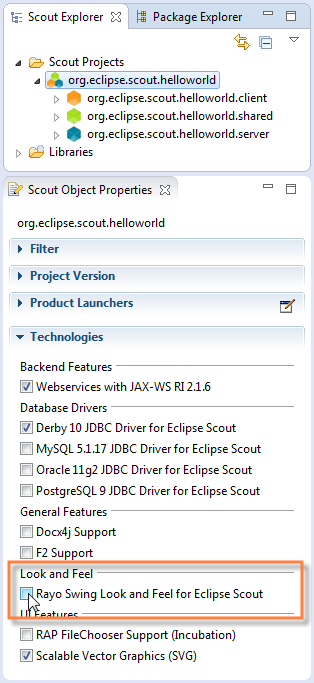
\includegraphics[width=6cm]{sdk_rayo_add_checkbox.png} \hspace{5mm}
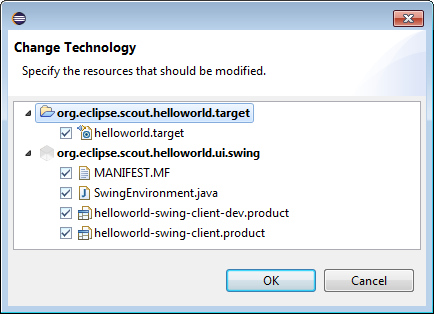
\includegraphics[width=7cm]{sdk_rayo_confirm_changes.png}
\caption{Adding the Rayo Swing look and feel. The Rayo checkbox to activate the look and feel is highlighted on the left hand side. The dialog on the right hand side shows the changes in the Swing plugin that will be made by the Scout SDK.}
\figlabel{selecting_rayo}
\end{figure}

To add Rayo in the Scout SDK to our ''Hello World'' project, switch to the Scout Explorer and select the top-level \node{org.eclipse.scout.helloworld}.
Then, according to \figref{selecting_rayo}, select the checkbox \element{Rayo Swing Look and Feel for Eclipse Scout} under the \element{Technologies} section of the Scout Object Properties.
This brings up a dialog showing the proposed changes to the Swing plugin of the ''Hello World'' application. 
These changes need to be confirmed with the \button{OK}.
The first time the user adds the Rayo feature in the Scout SDK, Eclipse needs to download the package from the Eclipse Marketplace\footnote{
Eclipse Marketplace: \url{http://marketplace.eclipse.org/}
}.
This download and subsequent installation of Rayo will make you to go through the following steps.

\begin{enumerate}
  \item Accept Licence: GPL with Classpath Exception
  \item Accept unsigned content
  \item Restart the Eclipse IDE
\end{enumerate}

In the last step we start the Swing client using the procedure described in \secref{run_initial}.
When we also start the web client of the ''Hello World'' application using the RAP product launcher, we can compare the result side by side.

Rayo has orignially been designed in 2009 by BSI for the desktop clients of its CRM\footnote{
CRM: Customer Relationship Management} 
and its contact center solutions.
Desktop and web application working with the same Rayo look and feel
On the deskop some synth classes needed to be adjusted. for this openjdk implementation was used. 
as a result, open sourcing of the adjusted synth clases under gpl with classpath exception was required
as this licence is not compatible with hosting the code at eclipse org, rayo is located on the eclipse marketplace.
with the classpath exception part of the licence, commercial usage of rayo is explicitly possible.
the only restriction beeing that modifications to the rayo package will have to be published under the same licence.

At the core of the Rayo Look and Feel lies Java Synth\footnote{
Java Synth Look and Feel: \url{http://en.wikipedia.org/wiki/Synth_Look_and_Feel}
}.
bla

\noindent Existing Documentation
\begin{itemize}
  \item wiki tutorial \url{http://wiki.eclipse.org/Scout/Tutorial/3.8/Rayo_Look_and_Feel}
\end{itemize}


% --------------------------------------------------------------------------- %
\section{Deploying to Tomcat}

As the final step of this ''Hello World'' tutorial we will deploy the Scout application to a Tomcat webserver.
First step: export war file(s)
Second step: deploy war file(s) to tomcat

Before we deploy the ''Hello World'' WAR files to the webserver you need a working Tomcat installation.
For this, you may want to read and follow the instructions provided in \appref{install_tomcat}.
As soon as you have a running Tomcat instance you can verify this in a web browser of your choice by typing \url{http://localhost:8080/} into its address bar.
You should then see the page shown on the left hand side of \figref{deploy_tomcat}.

\begin{figure}
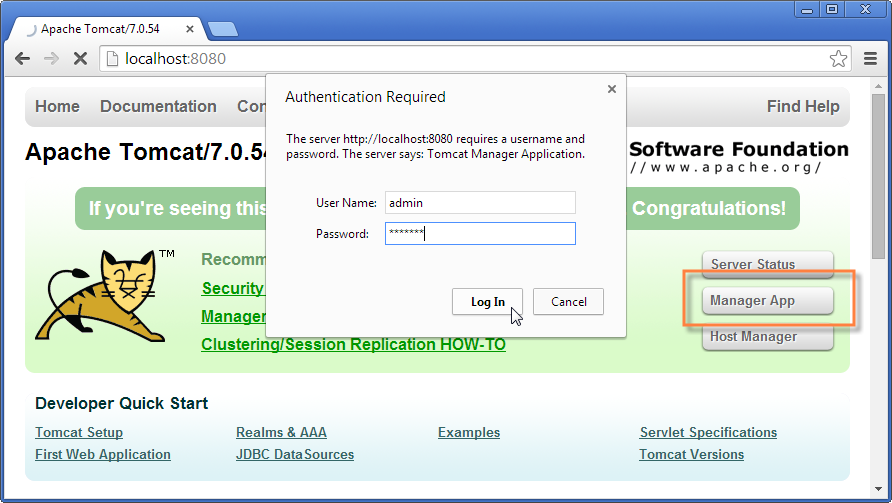
\includegraphics[width=7cm]{tomcat_managerapp_login.png} \hspace{5mm}
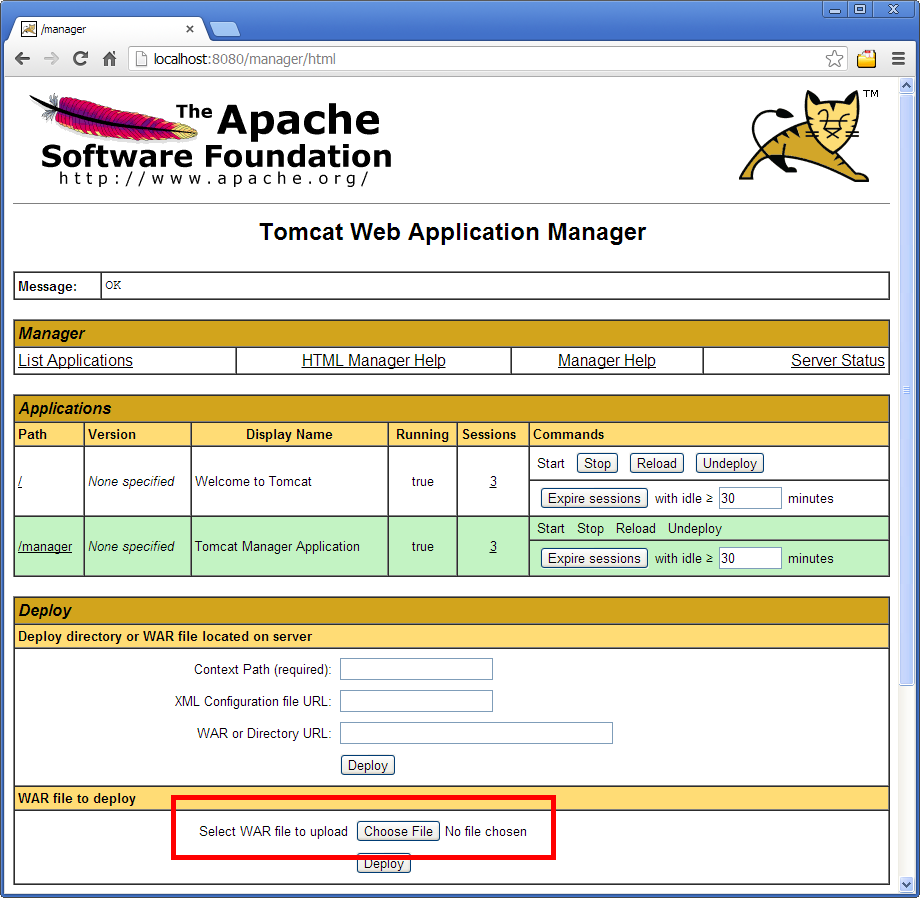
\includegraphics[width=7cm]{tomcat_managerapp_selectwar.png}
\caption{The login box after clicking the highlighted ''Manager App'' button. 
The WAR files to be deployed can then be selected using button ''Choose File'' highlighted on the right hand side}
\figlabel{deploy_tomcat}
\end{figure}

Once the web browser shows the successful running of your Tomcat instance you can switch to its ''Manager App'' by clicking on the button highlighted in \figref{deploy_tomcat}.
After entering user name and password you will then be shown Tomcat's manager application.
If you don't know the correct username or password you may look it up in the file \filename{tomcat-users.xml} according to \lstref{tomcat.users} located in subdirectory \filename{conf} of your Tomcat installation.
You may adapt the file's content to update passwords or add users.
The changes will then become effective after a restart of Tomcat.
For a rough overview of the organisation of the Tomcat installation directory also see \figref{tomcat.install.dir}.

\begin{lstlisting}[
  language=xml,
  float,
  label=\lstlabel{tomcat.users},
  caption=The content of the \texttt{tomcat-users.xml} file]
  <tomcat-users>
    <!--
    NOTE: By default, no user is included in the "manager-gui" role required
    to operate the "/manager/html" web application. If you wish to use it
    you must define such a user - the username and password are arbitrary.
    -->
	<user name="admin" password="s3cret" roles="manager-gui"/>
  </tomcat-users>	
\end{lstlisting}

\begin{figure}
\begin{verbatim}
  [Tomcat directory]
   |
   +-- conf
   |   +-- tomcat-users.xml
   |
   +-- webapps
       +-- helloworld
       |   +-- WEB-INF
       |   +-- ...
       +-- helloworld.war
\end{verbatim}
\caption{The organization of the Tomcat installation directory}
\figlabel{tomcat.install.dir}
\end{figure}

After logging successfully into Tomcats manager application, you can select the WAR file(s) to be deployed using button ''Choose File'' according to the right hand side of \figref{deploy_tomcat}.
After picking your WAR file and closing the file chooser, click on button ''Deploy'' (located below button ''Choose File'') to deploy the application to the Tomcat webserver.
This will copy the selected WAR file into Tomcats \filename{webapps} directory and unpack its content into a subdirectory with the same name.
Deploying the file \filename{helloworld.war} will extract its contents into a subdirectory named \filename{helloworld} as shown in \figref{tomcat.install.dir}.

ipconfig stuff

\begin{figure}
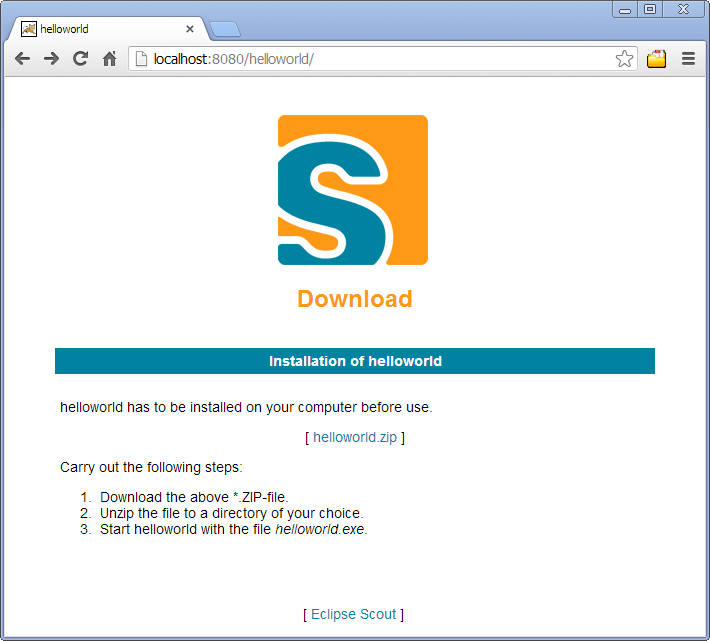
\includegraphics[width=10cm]{tomcat_helloworld_download.png}
\caption{The ''Hello World'' home page, providing a link to download the desktop client.}
\figlabel{helloworld_running_download}
\end{figure}

\begin{figure}
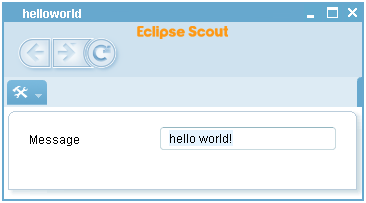
\includegraphics[width=4.5cm]{helloworld_finished_rayo_swing.png}\hspace{5mm}
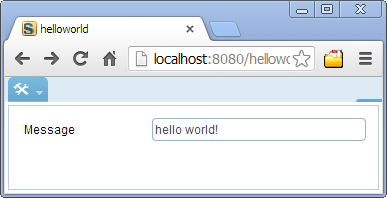
\includegraphics[width=4.5cm]{helloworld_finished_rayo_rap.png}\hspace{5mm}
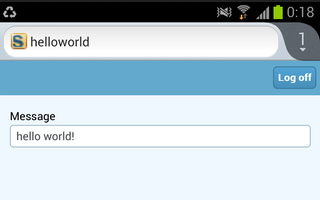
\includegraphics[width=4.5cm]{helloworld_finished_rayo_rap_mobile.png}
\caption{The ''Hello World'' client application running on the desktop, in the browser and on a mobile device.}
\figlabel{helloworld_running_clients}
\end{figure}

\noindent Existing Documentation
\begin{itemize}
  \item wiki tutorial: \url{http://wiki.eclipse.org/Scout/Tutorial/3.8/Deploy_to_Tomcat}
\end{itemize}

% --------------------------------------------------------------------------- %

\ifx\wholebook\relax\else
   \begin{thebibliography}{99}
  \addcontentsline{toc}{chapter}{Bibliography}
  
  % add/insert books in alphabetical order of 1st author
  
  \bibitem{batessierra05}
    \textit{Bert Bates, Kathy Sierra},
	\textbf{Head First Java} 2nd edition, 
	O'Reilly Media, 2005.

  \bibitem{bloch08} 
    \textit{Joshua Bloch},
    \textbf{Effective Java} 2nd edition, 
	Addison-Wesley, 2008.
	
  \bibitem{eckel06}
    \textit{Bruce Eckel},
	\textbf{Thinking in Java} 4th edition, 
	Prentice Hall International, 2006.

\end{thebibliography}

   \end{document}
\fi

% =========================================================================== %
